\section{Pure Soliton Case／纯孤子情形}
\EN{Here all reflection coefficients vanish, so only discrete data contribute to the potentials. This setting gives explicit soliton solutions. The discrete spectrum is the set $\mathcal Z$ of all poles of $M$ except zero. We impose suitable restrictions, formulate an RH problem, and show how its solution constructs soliton solutions of (1.1).}
\CN{反射系数全为零时，连续谱跳跃消失，只剩离散极点。下文对极点位置及留数施加特定限制，然后从相应 RH 问题重构解。}
\subsection{Pure Soliton RH Problem／纯孤子 RH 问题}
\EN{Since Assumptions 3.1 and 3.2 no longer hold, the behavior at zero differs significantly from the soliton-free case. There is no jump on $\Gamma$, and $M$ admits the Laurent expansion}
\CN{此时无跳跃，可跨射线粘合。原文采用至多一阶原点极点的 Laurent 展开}
\begin{equation}\originaleq{3.41}
M(x,t,k)=\sum\limits_{l=-1}^{\infty}\mathcal M^{(l)}(x,t)k^l.
\end{equation}
\begin{note}
“无跳跃”只保证穿孔邻域解析，本身不能排除高阶极点或本性奇点。因此 (3.41) 的下限 $-1$ 应视作此纯孤子 RH 模型的一项原点条件，不能仅由无跳跃推出。
\end{note}
\EN{Symmetry (3.46) requires the residue to satisfy}
\CN{比较循环及共轭对称中的 $k^{-1}$ 系数，得到}
\begin{equation}\originaleq{3.42}
A(-\ii\mathcal M^{(-1)})A^{-1}=\mathcal M^{(-1)},\qquad B\mathcal M^{*(-1)}B=\mathcal M^{(-1)}.
\end{equation}
\EN{Also $[M_1]_2=\mu_{+2}$. Combining (3.42) with (2.23), the residue has the form (3.43), where $\widetilde\delta_1,\widetilde\delta_2$ are scalar functions of $x,t$.}
\CN{第二列已由 Jost 原点展开确定；循环关系依次确定其他三列，得到}
\begin{equation}\originaleq{3.43}
\mathcal M^{(-1)}=\widetilde\delta_1\begin{pmatrix}\ii&0&\ii&0\\0&1&0&1\\-\ii&0&-\ii&0\\0&-1&0&-1\end{pmatrix}
+\widetilde\delta_2\begin{pmatrix}0&\ii&0&\ii\\1&0&1&0\\0&-\ii&0&-\ii\\-1&0&-1&0\end{pmatrix}.
\end{equation}
\EN{To complete the RH formulation, one must determine residue conditions at the poles. We have failed to derive these conditions directly, even with an explicit expression for $M$ such as (3.12). However, imposing the following conditions gives soliton solutions. We next describe the setting.}
\CN{原文坦言，尚未从一般散射公式直接导出离散留数条件，而是发现下面这组条件能产生孤子解。必须保留这个逻辑地位：它是特定逆问题的设定，并非已证明的一般离散谱分类。}
\EN{Assume all poles are simple. Restrict the poles of $M_1$ to $e^{\frac{\pi\ii}{4}}\mathbb R_+$ and denote them by $\mathcal Z_1=\{\zeta_j\}_{j=1}^N$. All other poles follow from the $A$ and $B$ symmetries. Define}
\CN{取互不相同的简单极点 $\zeta_j$ 位于第一象限的对角射线上，完整极点集为 $\mathcal Z=\pm\mathcal Z_1\cup\pm\ii\mathcal Z_1$。定义留数函数}
\begin{equation}\originaleq{3.44}
F_j(x,t)=\tau_j e^{(\theta_2-\theta_3)(x,t,\zeta_j)},\qquad \tau_j>0,\qquad \theta_i=\Theta_{ii}.
\end{equation}
\EN{We require the following residue conditions.}
\CN{规定四个对称极点上的留数为}
\begin{equation}\originaleq{3.45}
\begin{aligned}
\operatorname*{Res}_{k=\zeta_j}M&=\lim\limits_{k\to\zeta_j}M\begin{pmatrix}0&0&0&\ii F_j\\0&0&F_j&0\\0&0&0&0\\0&0&0&0\end{pmatrix},\\
\operatorname*{Res}_{k=\ii\zeta_j}M&=\lim\limits_{k\to\ii\zeta_j}M\begin{pmatrix}0&\ii F_j&0&0\\0&0&0&0\\0&0&0&0\\0&0&-F_j&0\end{pmatrix},\\
\operatorname*{Res}_{k=-\zeta_j}M&=\lim\limits_{k\to-\zeta_j}M\begin{pmatrix}0&0&0&0\\0&0&0&0\\0&-\ii F_j&0&0\\-F_j&0&0&0\end{pmatrix},\\
\operatorname*{Res}_{k=-\ii\zeta_j}M&=\lim\limits_{k\to-\ii\zeta_j}M\begin{pmatrix}0&0&0&0\\F_j&0&0&0\\0&0&0&-\ii F_j\\0&0&0&0\end{pmatrix}.
\end{aligned}
\end{equation}
\begin{proof}
这里证明四个条件之间的一致性，而不是从未给出的散射假设推导第一个条件。
若 $M(k)=AM(\ii k)A^{-1}$，在 $k=\zeta_j$ 附近变换变量 $z=\ii k$，留数因 $\dd z/\dd k=\ii$ 而乘 $1/\ii$；故在 $\ii\zeta_j$ 的留数右乘矩阵等于 $\ii A^{-1}(\text{首个矩阵})A$。
逐次作循环置换即得后面三个矩阵，最后第四次回到自身。
在 $\zeta_j=\kappa_je^{\frac{\pi\ii}{4}}$ 上，$\theta_2-\theta_3=-\sqrt2\kappa_j(x-2\kappa_j^2t)$ 为实数，因此 $F_j$ 实，且 $\zeta_j^*=-\ii\zeta_j$，共轭对称也与第四个条件相容。
每个右乘矩阵的平方均为零，保证 $M$ 的相应奇列只由正则列的值给出，右侧极限有意义。
\end{proof}
\EN{If the fundamental eigenfunction satisfies the foregoing discrete-data assumptions, it satisfies the following RH problem.}
\CN{这些条件组成以下纯孤子模型。}
\begin{note}[RH Problem 2／RH 问题 2（Pure soliton／纯孤子）]
\EN{Seek a $4\times4$ matrix function $M$ analytic on $\mathbb C\setminus(\{0\}\cup\mathcal Z)$, with the symmetries (3.46).}
\CN{寻找除原点及指定极点外解析的矩阵，满足}
\begin{equation}\originaleq{3.46}
M(k)=AM(\ii k)A^{-1}=BM^*(k^*)B.
\end{equation}
\EN{At infinity it has expansion (3.47), subject to (3.48).}
\CN{无穷远的展开与附加条件为}
\begin{align}
M&=I+\dfrac{M^{(1)}}{k}+\dfrac{M^{(2)}}{k^2}+O(k^{-3}),\originaleq{3.47}\\
M_{12}^{(1)}&=M_{13}^{(1)}=0,\qquad M_{13}^{(2)}=\dfrac{1}{2}\partial_xM_{44}^{(1)}.\originaleq{3.48}
\end{align}
\EN{Near zero it has the Laurent expansion (3.49), with the residue (3.50).}
\CN{原点至多一阶极点，留数具如下形状：}
\begin{align}
M&=\sum\limits_{l=-1}^\infty\mathcal M^{(l)}k^l,\originaleq{3.49}\\
\mathcal M^{(-1)}&=\widetilde\delta_1\begin{pmatrix}\ii&0&\ii&0\\0&1&0&1\\-\ii&0&-\ii&0\\0&-1&0&-1\end{pmatrix}
+\widetilde\delta_2\begin{pmatrix}0&\ii&0&\ii\\1&0&1&0\\0&-\ii&0&-\ii\\-1&0&-1&0\end{pmatrix}.\originaleq{3.50}
\end{align}
\EN{It satisfies the inverse-transpose identity (3.51), and its simple poles obey (3.45).}
\CN{逆转置及所有非零极点条件为}
\begin{equation}\originaleq{3.51}
JM(-k)J^{-1}=M^A(k)=(M^{-1}(k))^{\mathsf T},\qquad k\notin\{0\}\cup\mathcal Z,
\end{equation}
并满足 (3.45)。
\end{note}
\begin{note}
\EN{Remark 13. The fundamental eigenfunction has the expansion (3.52), with the same coefficient forms as in (2.20). Thus it satisfies the second equation of (3.48), which is used in Theorem 3.3.}
\CN{注 13：正散射产生的矩阵具有}
\begin{equation}\originaleq{3.52}
M=I+\dfrac{\mu_+^{[1]}(x,t)}{k}+\dfrac{\mu_+^{[2]}(x,t)}{k^2}+O(k^{-3}).
\end{equation}
由 $\mu_{+,13}^{[2]}=u/4$、$\partial_x\mu_{+,44}^{[1]}=u/2$，可知 (3.48) 的导数条件是必要的；它不是从循环对称性单独推出的。
\end{note}
\EN{We explain the appropriateness of the imposed residues by reconstructing solutions from this RH problem. First prove uniqueness, following the steps of Lemmas 3.6 and 3.7. Any solution has determinant one. If $M,\widetilde M$ are two solutions, study their quotient near zero. Symmetry (3.51) gives (3.53), with residue (3.54). The quotient is $O(k^{-1})$. The remaining issue is removability of the discrete poles, which is verified by the method in Theorem 3.3.}
\CN{原文在此以一段文字概述纯孤子 RH 解的唯一性，下面补齐非零极点消去这一步。}
\begin{align}
M^{-1}&=\sum\limits_{l=-1}^\infty\mathcal N^{(l)}k^l,\originaleq{3.53}\\
\mathcal N^{(-1)}&=-\widetilde\delta_1\begin{pmatrix}\ii&0&\ii&0\\0&1&0&1\\-\ii&0&-\ii&0\\0&-1&0&-1\end{pmatrix}
-\widetilde\delta_2\begin{pmatrix}0&\ii&0&\ii\\1&0&1&0\\0&-\ii&0&-\ii\\-1&0&-1&0\end{pmatrix}.\originaleq{3.54}
\end{align}
\begin{proof}[Proof／证明（纯孤子 RH 解的唯一性）]
在某个非零极点 $a$，暂把 (3.45) 对应的右乘矩阵称为 $C_a$；这是具有实际消极点作用的矩阵，且 $C_a^2=0$。
若 $M=M_{-1}/(k-a)+M_0+\cdots$，留数条件等价于 $M_{-1}=M_0C_a$、$M_{-1}C_a=0$。故
\[
M(k)\left(I-\dfrac{C_a}{k-a}\right)
\quad\text{在 }a\text{ 解析},\qquad
\det\left(I\pm\dfrac{C_a}{k-a}\right)=1.
\]
于是 $\det M$ 在所有非零极点可去。原点留数秩至多二，故行列式至多二阶极点；无穷远 (3.31) 给出 $\det M=1+O(k^{-3})$，照引理 3.6 得 $\det M=1$。
上式正则因子因而可逆。两个解的局部分解都含同一个右因子 $I+C_a/(k-a)$，在 $M\widetilde M^{-1}$ 中完全抵消，所以商在非零极点解析。
(3.50) 中两个系数矩阵的任意两两乘积均为零；结合 (3.54)，商在原点至多一阶极点。
无穷远一阶系数仍是标量乘 $\operatorname{diag}(1,-\ii,-1,\ii)$，遂可逐字应用 (3.34)--(3.37) 的论证；单位行列式迫使该标量为零，商恒为单位矩阵。
\end{proof}
\EN{We are now ready to reconstruct the potentials from RH problem 2.}
\CN{接下来证明这组 RH 条件足以产生 HScKdV 解。}
\begin{papertheoremen}
Suppose $M(x,t,k)$ solves the Pure soliton RH problem. The functions defined by (3.55) satisfy the HScKdV system (1.1). Moreover, $v$ obeys (3.56).
\end{papertheoremen}
\begin{papertheoremcn*}
纯孤子 RH 问题的解通过以下重构给出方程组的解，并满足相应平方恒等式。
\end{papertheoremcn*}
\begin{align}
u&=2\partial_x\lim\limits_{k\to\infty}k(M_{44}-1),\qquad
v=4\operatorname{Im}\left(\lim\limits_{k\to\infty}k^2M_{12}\right),\originaleq{3.55}\\
3v^2&=2\partial_t\lim\limits_{k\to\infty}k(M_{44}-1)-\dfrac{1}{2}u_{xx}+\dfrac{3}{2}u^2.\originaleq{3.56}
\end{align}
\begin{proof}
\EN{In the spirit of Zakharov and Shabat [33], define the matrix function}
\CN{使用 Zakharov--Shabat 的解析重构思路，定义}
\begin{equation}\originaleq{3.57}
\psi(x,t,k)=P(k)M(x,t,k)e^{\Theta(x,t,k)}.
\end{equation}
\EN{Away from zero and the discrete poles, $\psi_x\psi^{-1}$ is analytic, and}
\CN{直接求导得}
\begin{equation}\originaleq{3.58}
\psi_x\psi^{-1}=P(M_x+ML)e^\Theta e^{-\Theta}M^{-1}P^{-1}
=PM_xM^{-1}P^{-1}+PMLM^{-1}P^{-1}.
\end{equation}
\EN{Using (3.50), (3.53), $P,P^{-1}$ and symmetry (3.46), the original proof states that this logarithmic derivative is $O(1)$ at zero. We next remove the discrete poles. Define}
\CN{先补足原点可去性，再处理非零极点。沿用原文定义}
\begin{equation}\originaleq{3.59}
W=P^{-1}\psi=Me^\Theta.
\end{equation}
\proofstep{原点可去性的完整理由。}
$P$ 的常数项乘 (3.50) 的留数为零，因此 $\psi=PM e^\Theta$ 本身在原点解析。
循环对称作两次给出 $M(-k)=A^2M(k)A^2$，且 $P(-k)A^2=P(k)$，从而
\[
\psi(-k)=\psi(k)A^2.
\]
因此 $\psi_1+\psi_3,\psi_2+\psi_4$ 是偶解析列，$\psi_1-\psi_3,\psi_2-\psi_4$ 是奇解析列，后两者可被 $k$ 整除。
代入已经求出的 $P^{-1}$，$\psi P^{-1}$ 的四列恰为
\[
\dfrac{\psi_2+\psi_4}{2},\quad\dfrac{\psi_1+\psi_3}{2},\quad
\dfrac{\psi_4-\psi_2}{2k},\quad\dfrac{\psi_1-\psi_3}{2\ii k}.
\]
故 $\psi P^{-1}$ 在原点解析，且其行列式为 $\det M\det e^\Theta=1$，所以逆也解析。
由于 $P$ 不依赖 $x,t$，
\[
\psi_x\psi^{-1}=\partial_x(\psi P^{-1})(\psi P^{-1})^{-1},\qquad
\psi_t\psi^{-1}=\partial_t(\psi P^{-1})(\psi P^{-1})^{-1},
\]
两者在原点均解析。这比仅说“负次幂相消”更直接，也同时覆盖时间部分。
\EN{The symmetries of $W$ reduce the discrete-pole calculation to $\zeta_j$. Its residue conditions at $\zeta_j$ and $-\zeta_j$ become (3.60), (3.61).}
\CN{指数共轭恰好消掉 $F_j$ 的时空因子，得到常数留数矩阵：}
\begin{align}
\operatorname*{Res}_{k=\zeta_j}W&=\lim\limits_{k\to\zeta_j}W\begin{pmatrix}0&0&0&\ii\tau_j\\0&0&\tau_j&0\\0&0&0&0\\0&0&0&0\end{pmatrix},\originaleq{3.60}\\
\operatorname*{Res}_{k=-\zeta_j}W&=\lim\limits_{k\to-\zeta_j}W\begin{pmatrix}0&0&0&0\\0&0&0&0\\0&-\ii\tau_j&0&0\\-\tau_j&0&0&0\end{pmatrix}.\originaleq{3.61}
\end{align}
\EN{Differentiation shows that $W_x$ satisfies the same residue condition. Write its expansion at $\zeta_j$ and that of $W$ at $-\zeta_j$ as follows.}
\CN{因 $\tau_j$ 与时空无关，求导保持同一留数条件。原文把展开系数记为 $A_a,B_a,C_a,D_a$ 以及小写字母：}
\begin{equation}\originaleq{3.62}
W_x=\dfrac{1}{k-\zeta_j}\begin{pmatrix}0&0&\tau_j B_1&\ii\tau_j A_1\\0&0&\tau_j B_2&\ii\tau_j A_2\\0&0&\tau_j B_3&\ii\tau_j A_3\\0&0&\tau_j B_4&\ii\tau_j A_4\end{pmatrix}
+\begin{pmatrix}A_1&B_1&C_1&D_1\\A_2&B_2&C_2&D_2\\A_3&B_3&C_3&D_3\\A_4&B_4&C_4&D_4\end{pmatrix}+O(k-\zeta_j).
\end{equation}
\begin{equation}\originaleq{3.63}
W=\dfrac{1}{k+\zeta_j}\begin{pmatrix}-\tau_jd_1&-\ii\tau_jc_1&0&0\\-\tau_jd_2&-\ii\tau_jc_2&0&0\\-\tau_jd_3&-\ii\tau_jc_3&0&0\\-\tau_jd_4&-\ii\tau_jc_4&0&0\end{pmatrix}
+\begin{pmatrix}a_1&b_1&c_1&d_1\\a_2&b_2&c_2&d_2\\a_3&b_3&c_3&d_3\\a_4&b_4&c_4&d_4\end{pmatrix}+O(k+\zeta_j).
\end{equation}
\EN{Using (3.51), (3.59), (3.63) gives the inverse expansion at $\zeta_j$:}
\CN{逆转置对称把相反极点的展开转成}
\begin{equation}\originaleq{3.64}
\begin{aligned}
W^{-1}&=\dfrac{1}{k-\zeta_j}\begin{pmatrix}\tau_jd_1&\ii\tau_jd_2&-\tau_jd_3&-\ii\tau_jd_4\\\tau_jc_1&\ii\tau_jc_2&-\tau_jc_3&-\ii\tau_jc_4\\0&0&0&0\\0&0&0&0\end{pmatrix}\\
&\quad+\begin{pmatrix}a_1&\ii a_2&-a_3&-\ii a_4\\-\ii b_1&b_2&\ii b_3&-b_4\\-c_1&-\ii c_2&c_3&\ii c_4\\\ii d_1&-d_2&-\ii d_3&d_4\end{pmatrix}+O(k-\zeta_j).
\end{aligned}
\end{equation}
\EN{The original proof combines (3.62), (3.64) to show the absence of negative powers in $W_xW^{-1}$. Thus $\psi_x\psi^{-1}$ is entire and can be determined from infinity.}
\CN{不用继续增加系数简记即可补足相消：令 $C$ 为 (3.60) 的常数矩阵，$C^2=0$，则 $W(I-C/(k-\zeta_j))$ 是解析且行列式为一的矩阵。
局部写 $W=\bigl[W(I-C/(k-\zeta_j))\bigr](I+C/(k-\zeta_j))$；对 $x$ 或 $t$ 求导时右因子不变，故在 $W_xW^{-1}$、$W_tW^{-1}$ 中直接抵消。
其他极点由对称同理。两种对数导数均为整函数，且由大谱展开有多项式增长，所以 Cauchy 估计使它们为多项式。}
\EN{At infinity, $M$ and its inverse have the expansions (3.65), (3.66), with the coefficient forms in (3.31).}
\CN{无穷远展开为}
\begin{align}
M&=I+\dfrac{M^{(1)}}{k}+\dfrac{M^{(2)}}{k^2}+O(k^{-3}),\originaleq{3.65}\\
M^{-1}&=I-\dfrac{M^{(1)}}{k}+\dfrac{J^{-1}(M^{(2)})^{\mathsf T}J}{k^2}+O(k^{-3}).\originaleq{3.66}
\end{align}
\EN{Let $[C]_d$ and $[C]_o$ denote the diagonal and off-diagonal parts. Substitution into $PMLM^{-1}P^{-1}$ gives}
\CN{逐项展开，沿用原文四项分组：}
\begin{equation}\originaleq{3.67}
PMLM^{-1}P^{-1}=\Pi_1+\Pi_2+\Pi_3+\Pi_4+O(k^{-1}),
\end{equation}
\[
\begin{aligned}
\Pi_1&=PLP^{-1}=U^\infty,\\
\Pi_2&=P\dfrac{M^{(1)}}{k}LP^{-1}-P\dfrac{M^{(1)}}{k}LP^{-1}=0,\\
\Pi_3&=\dfrac{1}{k}P\left([M^{(2)}+(M^{(2)})^{\mathsf T}]_d-M^{(1)}M^{(1)}\right)JP^{-1},\\
\Pi_4&=\dfrac{1}{k}P[M^{(2)}+(M^{(2)})^{\mathsf T}]_oJP^{-1}.
\end{aligned}
\]
\EN{Comparing $k^{-2}$ in $MM^{-1}=I$ gives $\Pi_3=0$. Direct calculation also gives}
\CN{一阶系数与 $J$ 可交换，故第二项为零；逆矩阵恒等式给出第三项为零。空间导数项为}
\begin{equation}\originaleq{3.68}
PM_xM^{-1}P^{-1}=\partial_xM_{44}^{(1)}\begin{pmatrix}0&0&0&0\\0&0&0&0\\1&0&0&0\\0&1&0&0\end{pmatrix}+O(k^{-1}).
\end{equation}
\EN{As the logarithmic derivative is entire, the nonnegative part of its expansion is the function itself. Equations (3.67), (3.68) give (3.69), (3.70), which reduce to (3.71).}
\CN{整函数减去其多项式主部后在无穷远趋零，故由 Liouville 定理恒为零。原文将同一个等式分为相邻两行编号：}
\begin{align}
\psi_x\psi^{-1}&=U^\infty+\partial_xM_{44}^{(1)}\begin{pmatrix}0&0&0&0\\0&0&0&0\\1&0&0&0\\0&1&0&0\end{pmatrix}\originaleq{3.69}\\
&\quad+\begin{pmatrix}0&0&0&0\\0&0&0&0\\0&-1&0&1\\\ii&0&-\ii&0\end{pmatrix}
[M^{(2)}+(M^{(2)})^{\mathsf T}]_oJ
\begin{pmatrix}0&\dfrac{1}{2}&0&0\\\dfrac{1}{2}&0&0&0\\0&\dfrac{1}{2}&0&0\\\dfrac{1}{2}&0&0&0\end{pmatrix}.\originaleq{3.70}
\end{align}
\begin{equation}\originaleq{3.71}
\psi_x\psi^{-1}=U^\infty+\begin{pmatrix}
0&0&0&0\\0&0&0&0\\
\partial_xM_{44}^{(1)}+2M_{13}^{(2)}&2\ii(M_{12}^{*(2)}-M_{12}^{(2)})&0&0\\
2\ii(M_{12}^{*(2)}-M_{12}^{(2)})&\partial_xM_{44}^{(1)}+2M_{13}^{(2)}&0&0
\end{pmatrix}.
\end{equation}
\EN{Using (3.48), this is the $x$-part of (2.1) with the reconstructed $u,v$. Analogous arguments give the $t$-part. Substitution into (1.1) then yields (3.56).}
\CN{由 (3.48)，左下块对角元为 $2\partial_xM_{44}^{(1)}=u$，非对角元为 $4\operatorname{Im}M_{12}^{(2)}=v$，得到空间 Lax 矩阵。}
\proofstep{补足时间部分的计算及正则性前提。}
RH 解须随 $(x,t)$ 至少具有下列求导所需的光滑性。有限极点模型可将问题化为有限维线性系统；在该系统可逆的开集，系数光滑且解也光滑，所以这一前提可直接核验。
已经证明 $\psi_t\psi^{-1}$ 在所有有限谱点解析。其无穷远表达为
\[
\psi_t\psi^{-1}=PM_tM^{-1}P^{-1}+PMZM^{-1}P^{-1},\qquad Z=2k^3J^3.
\]
为复现时间计算，可把 $M=I+\displaystyle\sum\limits_{r\geq1}M^{(r)}k^{-r}$、$M^{-1}=I+\displaystyle\sum\limits_{r\geq1}(M^{-1})^{(r)}k^{-r}$ 代入。
逆系数由 $MM^{-1}=I$ 逐阶给出；空间方程给出
\[
[J,M^{(r+1)}]=\partial_xM^{(r)}-\dfrac{u\Lambda_1+v\Lambda_2}{2}M^{(r-1)},\quad r\geq1,
\qquad [J,M^{(1)}]=0.
\]
非对角条目除以 $J_{aa}-J_{bb}$，对角条目保留其导数；只需计算至 $r=3$，因为 $Z$ 为三次、$P$ 的最高次数为一，所有更高阶仅贡献负次幂。
例如三阶系数中实际用到的独立非对角条目为
\[
\begin{aligned}
M_{12}^{(3)}&=\dfrac{v_x-(1+\ii)M_{44}^{(1)}v}{4},\\
M_{13}^{(3)}&=\dfrac{\ii(2M_{44}^{(1)}u-u_x)}8,\\
M_{24}^{(3)}&=-\dfrac{M_{44}^{(1)}u}4+\dfrac{u_x}{8}.
\end{aligned}
\]
其余非对角条目由 $M^{(3)}=\ii A M^{(3)}A^{-1}=BM^{*(3)}B$ 得到；四阶非对角条目逐个由
$\displaystyle M_{ab}^{(4)}=(\partial_xM_{ab}^{(3)}-\sum\limits_c(\widetilde U_2)_{ac}M_{cb}^{(2)})/(J_{aa}-J_{bb})$ 给出。
对角的 $M^{(3)},M^{(4)}$ 与 $J^3$ 可交换，其在线性最高项中消去，故不需要另取不定积分。
将这些式子与逆矩阵递推代入，\textbf{尚未使用 PDE} 时，时间多项式四行依次为
\[
\begin{aligned}
\psi_t\psi^{-1}&=\begin{pmatrix}
\dfrac{u_x}{2}&-v_x&2k^2-u&2v\\
-v_x&\dfrac{u_x}{2}&2v&-2k^2-u\\
2k^4+k^2u&-v_{xx}+uv&-\dfrac{u_x}{2}&v_x\\
-v_{xx}+uv&2k^4-k^2u&v_x&-\dfrac{u_x}{2}
\end{pmatrix}\\
&\quad+\left(\partial_tM_{44}^{(1)}+\dfrac{u_{xx}}{4}-\dfrac{u^2}{4}+\dfrac{v^2}{2}\right)
\begin{pmatrix}0&0&0&0\\0&0&0&0\\1&0&0&0\\0&1&0&0\end{pmatrix}.
\end{aligned}
\]
这里必须保留 $\partial_tM_{44}^{(1)}$，不能提前把目标 PDE 代进去而形成循环论证。
令 $U=\psi_x\psi^{-1}$，$V=\psi_t\psi^{-1}$，混合偏导相等自动给出零曲率。
其 $(1,1)$ 项不含 $u_t,v_t$，逐项相乘为
\[
0=-\dfrac{u_{xx}}2+
\left(\partial_tM_{44}^{(1)}+\dfrac{u_{xx}}4-\dfrac{u^2}{4}+\dfrac{v^2}{2}\right)
+u^2-2v^2
=\partial_tM_{44}^{(1)}-\dfrac{u_{xx}}4+\dfrac{3u^2}{4}-\dfrac{3v^2}{2}.
\]
所以 $\partial_tM_{44}^{(1)}=u_{xx}/4-3u^2/4+3v^2/2$，这已经给出 (3.56)。代回时间矩阵，公共项变成 $u_{xx}/2+2v^2-u^2$，恰为第 2.1 节校正的 $V$。
剩下的 $(3,1)$、$(3,2)$ 零曲率条目由第 2.1 节的逐元素计算分别给出 (1.1) 的两条 PDE，完成反向重构证明。
\end{proof}
\begin{note}
\EN{Remark 14. The second equation in (3.48) is required in the proof. The next subsection shows that it is not important in calculating explicit soliton solutions, but we have no way to remove the condition.}
\CN{注 14：作者不能从抽象定理中去掉 (3.48) 的导数条件。后面的行向量计算简化了求显式解的过程，却不自动证明任意行向量解都能提升为满足全部条件的矩阵解；显式解最后仍应直接核验 PDE。}
\end{note}
\subsection{Soliton Solutions／孤子解}
\EN{Theorem 3.3 reconstructs solutions once RH problem 2 is solved. Solving the $4\times4$ matrix problem directly is complicated, especially because of the singularity at zero. Introduce the row vector}
\CN{用固定行向量求和消去原点留数，降低显式求解的维数：}
\begin{equation}\originaleq{3.72}
n(x,t,k)=(1,1,1,1)M(x,t,k).
\end{equation}
\EN{The following lemma summarizes the properties of $n$.}
\CN{行向量满足以下性质。}
\begin{paperlemmaen}
If $M$ solves the pure soliton RH problem, the row vector (3.72) is analytic off $\{0\}\cup\mathcal Z$, satisfies (3.73), is normalized by (3.74), is $O(1)$ at zero, obeys the residues (3.75), and reconstructs the potentials by (3.76), (3.77).
\end{paperlemmaen}
\begin{paperlemmacn*}
行向量继承解析性、对称性和留数条件，原点奇性消失；它的一阶无穷远系数足以重构 $u$ 与 $v^2$。
\end{paperlemmacn*}
\begin{align}
n(x,t,k)&=n(x,t,\ii k)A^{-1}=n^*(x,t,k^*)B,\originaleq{3.73}\\
n(x,t,k)&=(1,1,1,1)+O(k^{-1}),\qquad k\to\infty.\originaleq{3.74}
\end{align}
\begin{equation}\originaleq{3.75}
\begin{aligned}
\operatorname*{Res}_{k=\zeta_j}n&=\lim\limits_{k\to\zeta_j}n\begin{pmatrix}0&0&0&\ii F_j\\0&0&F_j&0\\0&0&0&0\\0&0&0&0\end{pmatrix},\\
\operatorname*{Res}_{k=\ii\zeta_j}n&=\lim\limits_{k\to\ii\zeta_j}n\begin{pmatrix}0&\ii F_j&0&0\\0&0&0&0\\0&0&0&0\\0&0&-F_j&0\end{pmatrix},\\
\operatorname*{Res}_{k=-\zeta_j}n&=\lim\limits_{k\to-\zeta_j}n\begin{pmatrix}0&0&0&0\\0&0&0&0\\0&-\ii F_j&0&0\\-F_j&0&0&0\end{pmatrix},\\
\operatorname*{Res}_{k=-\ii\zeta_j}n&=\lim\limits_{k\to-\ii\zeta_j}n\begin{pmatrix}0&0&0&0\\F_j&0&0&0\\0&0&0&-\ii F_j\\0&0&0&0\end{pmatrix}.
\end{aligned}
\end{equation}
\begin{align}
u(x,t)&=2\partial_x\lim\limits_{k\to\infty}k(n_4-1),\originaleq{3.76}\\
3v^2(x,t)&=2\partial_t\lim\limits_{k\to\infty}k(n_4-1)-\dfrac{1}{2}u_{xx}+\dfrac{3}{2}u^2.\originaleq{3.77}
\end{align}
\begin{proof}
\EN{The proof is almost obvious. The new reconstruction formulas hold because $M^{(1)}$ is diagonal.}
\CN{补齐各项：常行向量左乘保持解析性与留数。它左乘 $A,B$ 都不变，所以保留 (3.73)；左乘单位阵给出归一化。
(3.50) 每列分量之和为零，故 $n$ 的原点留数为零；有限极点模型中由可去奇点定理可解析补上原点。
由于 $M^{(1)}$ 对角，$n_4$ 的 $k^{-1}$ 系数恰为 $M_{44}^{(1)}$，故重构式与 (3.55)、(3.56) 一致。}
\end{proof}
\EN{The conditions of Lemma 3.8 form an exactly solvable linear system. Take $N=1$, with $\zeta_1=\kappa_1e^{\frac{\pi\ii}{4}}$, $\kappa_1>0$, and $\tau_1>0$. The original text states that $\tau_1<0$ corresponds to singular solitons and restricts to the positive case. The residues and normalization give}
\CN{以单个基本离散谱点为例。按留数列结构，第四分量只有 $-\ii\zeta_1$ 与 $\zeta_1$ 两个极点；扣去这两个主部后为整函数，在无穷远趋一，由 Liouville 定理得到}
\begin{equation}\originaleq{3.78}
\begin{aligned}
n_4(k)&=1-\dfrac{\ii F_1}{k+\ii\zeta_1}n_3(-\ii\zeta_1)+\dfrac{\ii F_1}{k-\zeta_1}n_1(\zeta_1)\\
&=1-\dfrac{\ii F_1}{k+\ii\zeta_1}n_3(-\ii\zeta_1)+\dfrac{\ii F_1}{k-\ii\zeta_1^*}n_1(\ii\zeta_1^*).
\end{aligned}
\end{equation}
\EN{The symmetries give $n_3(-\ii\zeta_1)=n_4(-\zeta_1)$ and $n_1(\ii\zeta_1^*)=n_4(-\zeta_1^*)$. Thus}
\CN{利用循环对称把正则列的值全部换成第四分量：}
\begin{equation}\originaleq{3.79}
n_4(k)=1-\dfrac{\ii F_1}{k+\ii\zeta_1}n_4(-\zeta_1)+\dfrac{\ii F_1}{k-\ii\zeta_1^*}n_4(-\zeta_1^*).
\end{equation}
\EN{Evaluate this at $-\zeta_1,-\zeta_1^*$ and let $X=(n_4(-\zeta_1),n_4(-\zeta_1^*))^{\mathsf T}$. The resulting algebraic system is}
\CN{这两个点都不是 $n_4$ 的极点，可以直接代入。沿用原文的唯一辅助未知向量 $X$：}
\begin{equation}\originaleq{3.80}
X=\begin{pmatrix}
\dfrac{-\ii F_1}{-\zeta_1+\ii\zeta_1}&\dfrac{\ii F_1}{-\zeta_1-\ii\zeta_1^*}\\
\dfrac{-\ii F_1}{-\zeta_1^*+\ii\zeta_1}&\dfrac{\ii F_1}{-\zeta_1^*-\ii\zeta_1^*}
\end{pmatrix}X+\begin{pmatrix}1\\1\end{pmatrix}.
\end{equation}
\EN{This determines $n_4$, and the symmetries determine the entire row vector. The reconstruction formula gives}
\CN{求解二阶线性系统即可得到 $n_4$。大谱参数首项是两个留数之和，故}
\begin{equation}\originaleq{3.81}
u=2\partial_x\left(\ii F_1n_4(-\zeta_1^*)-\ii F_1n_4(-\zeta_1)\right).
\end{equation}
\EN{Solving (3.80) and substituting into (3.81), we obtain (3.82), with $x_0=\ln(\sqrt{\tau_1}/(2\kappa_1))\in\mathbb R$. Substitution into (3.77) gives (3.83).}
\CN{原文所列单孤子公式如下（位移常数及第二式自变量的校勘紧随其后）：}
\begin{align}
u(x,t)&=-4\kappa_1^2\operatorname{sech}^2\left(\sqrt2\kappa_1(x-2\kappa_1^2t)-x_0\right),\originaleq{3.82}\\
v(x,t)&=\pm2\sqrt2\kappa_1^2\operatorname{sech}\left(\sqrt2(x-2\kappa_1^2t)-x_0\right).\originaleq{3.83}
\end{align}
\EN{Thus the one-soliton solution is the following pair, consistent with the form in [1].}
\CN{原文在紧接着的最终联立式中已把第二个自变量补上 $\kappa_1$，写为}
\[
\begin{cases}
u=-4\kappa_1^2\operatorname{sech}^2\left(\sqrt2\kappa_1(x-2\kappa_1^2t)-x_0\right),\\
v=\pm2\sqrt2\kappa_1^2\operatorname{sech}\left(\sqrt2\kappa_1(x-2\kappa_1^2t)-x_0\right).
\end{cases}
\]
\begin{note}
(3.83) 漏印 $\kappa_1$，后面的最终联立式正确。由定义 (3.44) 实际解出 (3.80) 后，位移应为 $x_0=\log(\tau_1/(2\kappa_1))$；原文 $\sqrt{\tau_1}$ 与所定义的 $F_1$ 不符。若把 $x_0$ 当任意实参数，孤子族本身不受这项参数命名误差影响。
原文关于负 $\tau_1$ 必然导致奇性的判断也不能由本系统推出：下列行列式为 $1+F_1^2/(4\kappa_1^2)>0$，对实负 $F_1$ 仍不为零。本笔记沿用作者选择的正参数，但不复述为已证的奇性结论。
\end{note}
\begin{proof}[Proof／证明（从代数系统到双分量孤子）]
\proofstep{一：化简两阶系统，不改变原参数。}
代入 $\zeta_1=(1+\ii)\kappa_1/\sqrt2$，(3.80) 右端系数矩阵为
\[
\begin{pmatrix}
\dfrac{\ii F_1}{\sqrt2\kappa_1}&-\dfrac{(1+\ii)F_1}{2\sqrt2\kappa_1}\\
-\dfrac{(1-\ii)F_1}{2\sqrt2\kappa_1}&-\dfrac{\ii F_1}{\sqrt2\kappa_1}
\end{pmatrix}.
\]
将其移到左侧，行列式是 $1+F_1^2/(4\kappa_1^2)$。两次 Cramer 展开给出
\[
\begin{aligned}
n_4(-\zeta_1)&=\dfrac{\kappa_1(4\kappa_1+\sqrt2F_1(-1+\ii))}{F_1^2+4\kappa_1^2},\\
n_4(-\zeta_1^*)&=\dfrac{\kappa_1(4\kappa_1-\sqrt2F_1(1+\ii))}{F_1^2+4\kappa_1^2}.
\end{aligned}
\]
因而
\[
\lim\limits_{k\to\infty}k(n_4-1)
=\ii F_1\bigl(n_4(-\zeta_1^*)-n_4(-\zeta_1)\bigr)
=\dfrac{2\sqrt2\kappa_1F_1^2}{F_1^2+4\kappa_1^2}.
\]
由相位 $F_1=\tau_1e^{-\sqrt2\kappa_1(x-2\kappa_1^2t)}$，有 $\partial_xF_1=-\sqrt2\kappa_1F_1$，故
\[
u=-\dfrac{64\kappa_1^4F_1^2}{(F_1^2+4\kappa_1^2)^2}
=-4\kappa_1^2\operatorname{sech}^2\left(\sqrt2\kappa_1(x-2\kappa_1^2t)-\log\dfrac{\tau_1}{2\kappa_1}\right).
\]
最后一步用 $\operatorname{sech}^2 s=4e^{-2s}/(1+e^{-2s})^2$，没有重新定义任何谱参数。
\proofstep{二：确定 $v$，并说明符号。}
将上面的有理式对 $t$ 求导并代入 (3.77)，约分得到
\[
v^2=\dfrac{128\kappa_1^6F_1^2}{(F_1^2+4\kappa_1^2)^2}
=8\kappa_1^4\operatorname{sech}^2\left(\sqrt2\kappa_1(x-2\kappa_1^2t)-\log\dfrac{\tau_1}{2\kappa_1}\right).
\]
所以取全局一致的正号或负号都给出所列孤子。若需从特定矩阵解确定符号，使用 (3.55) 的二阶虚部；仅凭平方公式不能指定它。
\proofstep{三：直接代回原方程，独立于矩阵存在性。}
为写清导数，仅在本段把完整相位写成 $s=\sqrt2\kappa_1(x-2\kappa_1^2t)-x_0$；这是实际链式法则变量，不是压缩矩阵计算的简记。
恒等式 $\partial_s\operatorname{sech}s=-\operatorname{sech}s\tanh s$、$\partial_s\tanh s=\operatorname{sech}^2s$ 给出
\[
v_{xx}=2\kappa_1^2v-4\kappa_1^2v\operatorname{sech}^2s=(2\kappa_1^2+u)v,
\quad
v_{xxx}=2\kappa_1^2v_x+u_xv+uv_x.
\]
又 $u_xv=2uv_x$，故
\[
-v_{xxx}+3uv_x=-2\kappa_1^2v_x-u_xv+2uv_x=-2\kappa_1^2v_x=v_t.
\]
对第一分量，直接求二阶导数有
\[
u_{xx}=8\kappa_1^2u+3u^2,\qquad v^2=-2\kappa_1^2u.
\]
求第一式空间导数、第二式空间导数，得到
\[
\dfrac{1}{2}u_{xxx}-3uu_x+6vv_x
=4\kappa_1^2u_x+3uu_x-3uu_x-6\kappa_1^2u_x
=-2\kappa_1^2u_x=u_t.
\]
两条方程均严格成立。函数及任意空间导数指数下降，故每个固定时刻属 Schwartz 空间，任意有界时间区间也有统一 Schwartz 界。
\end{proof}
\begin{figure}[htbp]
\centering
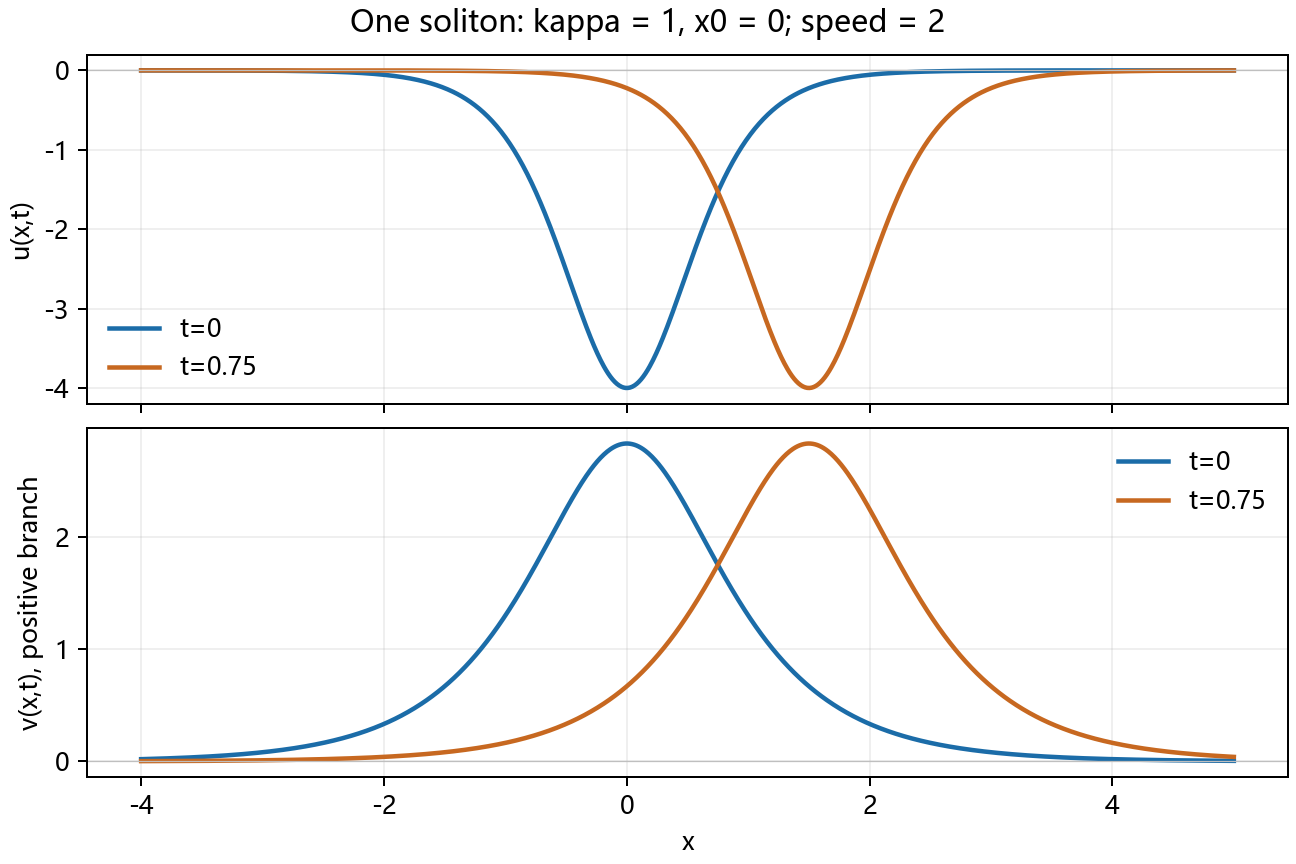
\includegraphics[width=0.94\textwidth]{figures/one-soliton.png}
\caption*{\textbf{Supplementary Figure S3.1／补充图 S3.1.} One soliton with $\kappa_1=1$, $x_0=0$ at two times.
同一个单孤子在 $t=0$ 与 $t=0.75$ 的两分量剖面；取 $v$ 的正号。中心由 0 移到 1.5，与速度 $2\kappa_1^2=2$ 一致。图由已核验的显式公式计算。}
\end{figure}
